\documentclass[a4paper, fleqn]{article}
\usepackage[utf8]{inputenc}
\usepackage{amsmath}
\usepackage{amssymb}
\usepackage{caption}
\usepackage{mathtools}
\usepackage{amsfonts}
\usepackage{lastpage}
\usepackage{tikz}
\usepackage{float}
\usepackage{textcomp}
\usetikzlibrary{patterns}
\usepackage{pdfpages}
\usepackage{gauss}
\usepackage{fancyvrb}
\usepackage[table]{colortbl}
\usepackage{fancyhdr}
\usepackage{graphicx}
\usepackage[margin=2.5 cm]{geometry}

\setlength\parindent{0pt}
\setlength\mathindent{75pt}

\definecolor{listinggray}{gray}{0.9}
\usepackage{listings}
\lstset{
	language=,
	literate=
		{æ}{{\ae}}1
		{ø}{{\o}}1
		{å}{{\aa}}1
		{Æ}{{\AE}}1
		{Ø}{{\O}}1
		{Å}{{\AA}}1,
	backgroundcolor=\color{listinggray},
	tabsize=3,
	rulecolor=,
	basicstyle=\scriptsize,
	upquote=true,
	aboveskip={0.2\baselineskip},
	columns=fixed,
	showstringspaces=false,
	extendedchars=true,
	breaklines=true,
	prebreak =\raisebox{0ex}[0ex][0ex]{\ensuremath{\hookleftarrow}},
	frame=single,
	showtabs=false,
	showspaces=false,
	showlines=true,
	showstringspaces=false,
	identifierstyle=\ttfamily,
	keywordstyle=\color[rgb]{0,0,1},
	commentstyle=\color[rgb]{0.133,0.545,0.133},
	stringstyle=\color[rgb]{0.627,0.126,0.941},
  moredelim=**[is][\color{blue}]{@}{@},
}

\lstdefinestyle{base}{
  emptylines=1,
  breaklines=true,
  basicstyle=\ttfamily\color{black},
}

\pagestyle{fancy}
\def\checkmark{\tikz\fill[scale=0.4](0,.35) -- (.25,0) -- (1,.7) -- (.25,.15) -- cycle;}
\newcommand*\circled[1]{\tikz[baseline=(char.base)]{
            \node[shape=circle,draw,inner sep=2pt] (char) {#1};}}
\newcommand*\squared[1]{%
  \tikz[baseline=(R.base)]\node[draw,rectangle,inner sep=0.5pt](R) {#1};\!}
\newcommand{\comment}[1]{%
  \text{\phantom{(#1)}} \tag{#1}}
\def\el{[\![}
\def\er{]\!]}
\def\dpip{|\!|}
\def\MeanN{\frac{1}{N}\sum^N_{n=1}}
\cfoot{Page \thepage\ of \pageref{LastPage}}
\DeclareGraphicsExtensions{.pdf,.png,.jpg}

\author{Nikolaj Dybdahl Rathcke (Student ID: 74763954)}
\title{Combinatorics (MATH429) \\ Assignment 3}
\lhead{Combinatorics (MATH429)}
\rhead{Assignment 3}

\begin{document}
\maketitle

\section*{Question 1}
The graph $G_1$ so that $M(G_1)\cong M_1$ is given in Figure \ref{fig2}:
\begin{figure}[H]
  \centering
  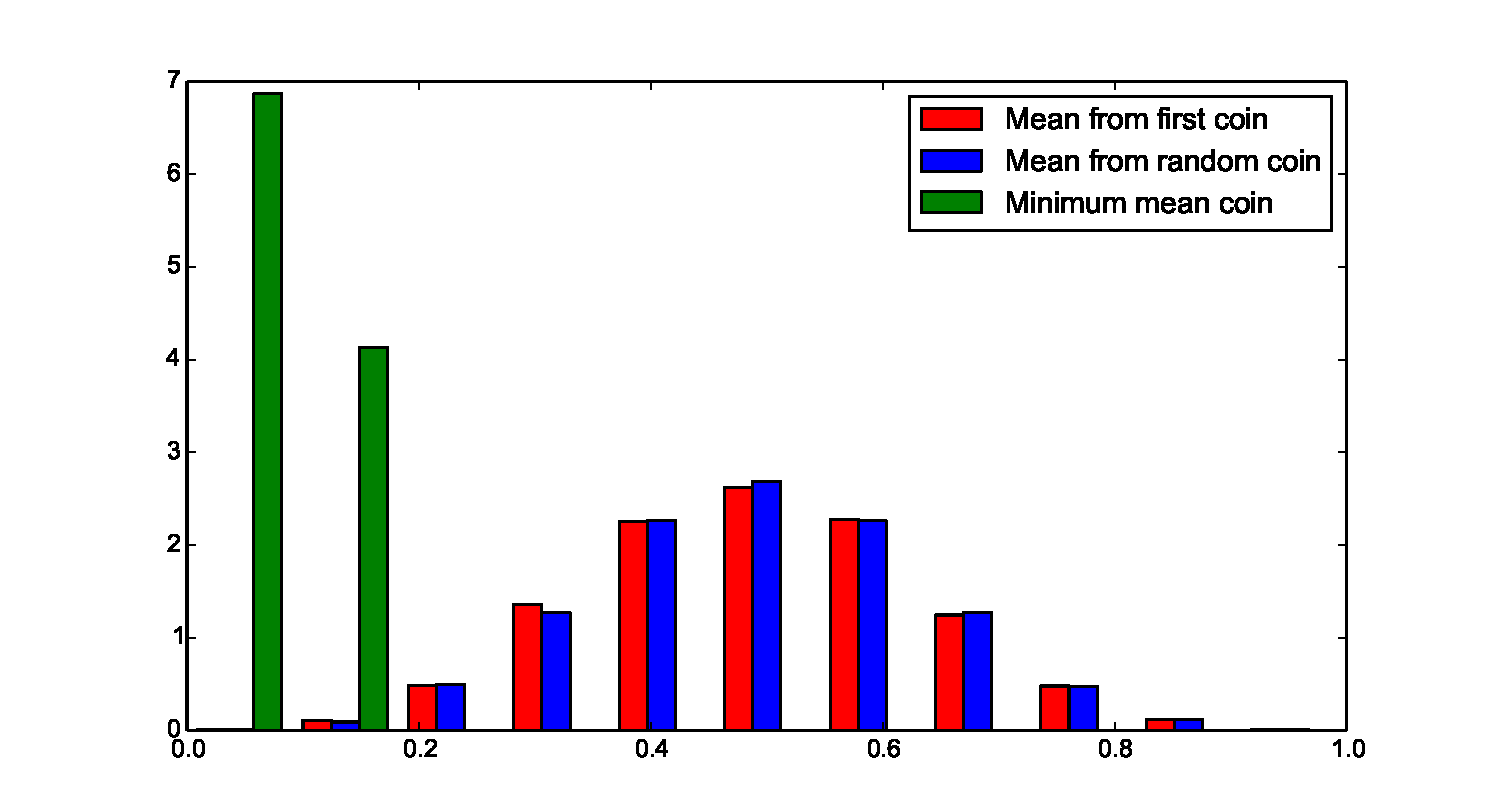
\includegraphics[scale=1]{fig2}
  \caption{A graph whose matroid is congruent to matroid given by the its representation
  $M_1$.}
  \label{fig2}
\end{figure}
To see this is true, note that we have three circuits of size $4$, that is, the sets
$\{1,2,4,5\},\{1,3,4,6\}$ and $\{2,3,5,6\}$. The graph only contains these three cycles
as well. Any set which contains one of these subset will be a cycle as well, while any
other set will not as it shouldn't. \\
The graph for $M_2$ is given in Figure \ref{fig3}:
\begin{figure}[H]
  \centering
  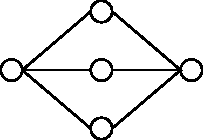
\includegraphics[scale=1]{fig3}
  \caption{The graph $G_2$ whose matroid is congruent to the one depicted in $M_2$.}
  \label{fig3}
\end{figure}
The geometric representation has $3$ lines with three points on them. These circuits are
$\{1,2,3\}, \{1,7,8\}$ and $\{5,6,7\}$ which are also the only cycles of length $3$ in the
graph. Furthermore, there are $5$ sets of circuits with size $4$. These are
$\{1,2,4,5\},\{1,5,6,8\},\{2,3,7,8\},\{2,4,6,8\}$ and $\{3,4,6,7\}$. The set
$\{1,5,6,8\}$ does not look like it is on a plane, but there is a plane spanned by
$\{1,8,7\}$ and $\{5,6,7\}$, so it must be.

\section*{Question 2}
To find the geometric representation, we start off by finding the dependent sets. We find
that the three element circuits of $A_1$, named $C_3$, are:
\begin{align*}
  C_3&=\{\{a,b,e\},\{a,d,h\},\{b,c,f\},\{c,d,g\},\{e,g,i\},\{f,h,i\}\}
\end{align*}
The sets of four elements that are dependent (and a circuit) are:
\begin{align*}
  C_4=\{&\{a,b,g,i\},\{a,c,e,f\},\{a,c,g,h\},\{a,d,f,i\}, \\
        &\{b,c,h,i\},\{b,d,e,h\},\{b,d,f,g\},\{c,d,e,i\},\{e,g,f,h\}\}
\end{align*}
a:
\begin{figure}[H]
  \centering
  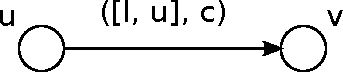
\includegraphics[scale=1]{fig6}
  \caption{Geometric representation of the vector matroid $A_1$.}
  \label{fig6}
\end{figure}
Note that $b$ and $d$ have the same height (so that $\{b,d,e,h\}$ is on a plane). The
line from $a$ to $i$ indicates $a$ is above $c$ so we have $\{a,c,e,f\}$ and
$\{a,c,g,h\}$ on a plane. The dashed lines mean they do not go straight up, but is
bended. This should include all the dependent sets of size $3$ and $4$ and not any ones
that are not dependent. \\
The circuits of size $3$ for $A_2$ are:
\begin{align*}
  C'_3=\{&\{a,b,f\},\{a,c,e\},\{a,d,g\},\{b,c,d\},\{e,f,g\}\}
\end{align*}
And the circuits of of four elements (anything that does not include a circuit of size
$3$):
\begin{align*}
  C'_4=\{&\{a,b,c,g\},\{a,b,d,e\},\{a,b,e,g\},\{a,c,d,f\},\{a,c,f,g\},\{a,d,e,f\}, \\
         &\{b,c,e,f\},\{b,c,e,g\},\{b,c,f,g\},\{b,d,e,f\},\{b,d,e,g\},\{b,d,f,g\}, \\
         &\{c,d,e,f\},\{c,d,e,g\},\{c,d,f,g\}\}
\end{align*}
The geometric representation is given by:
\begin{figure}[H]
  \centering
  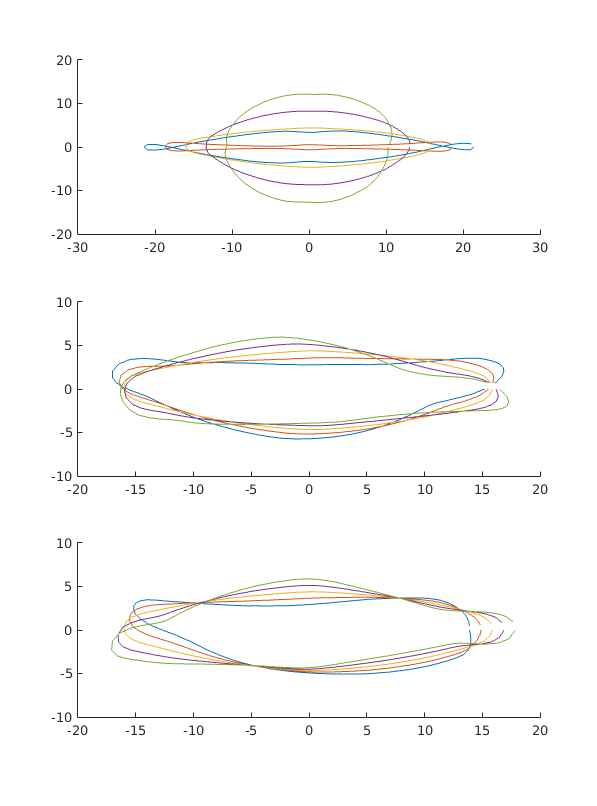
\includegraphics[scale=1]{fig5}
  \caption{Geometric representation of the vector matroid $A_2$.}
  \label{fig5}
\end{figure}
which we can verify have the circuits stated above.

\section*{Question 3}
\subsection*{(a)}
The bipartite graph is seen in Figure \ref{fig1}:
\begin{figure}[H]
  \centering
  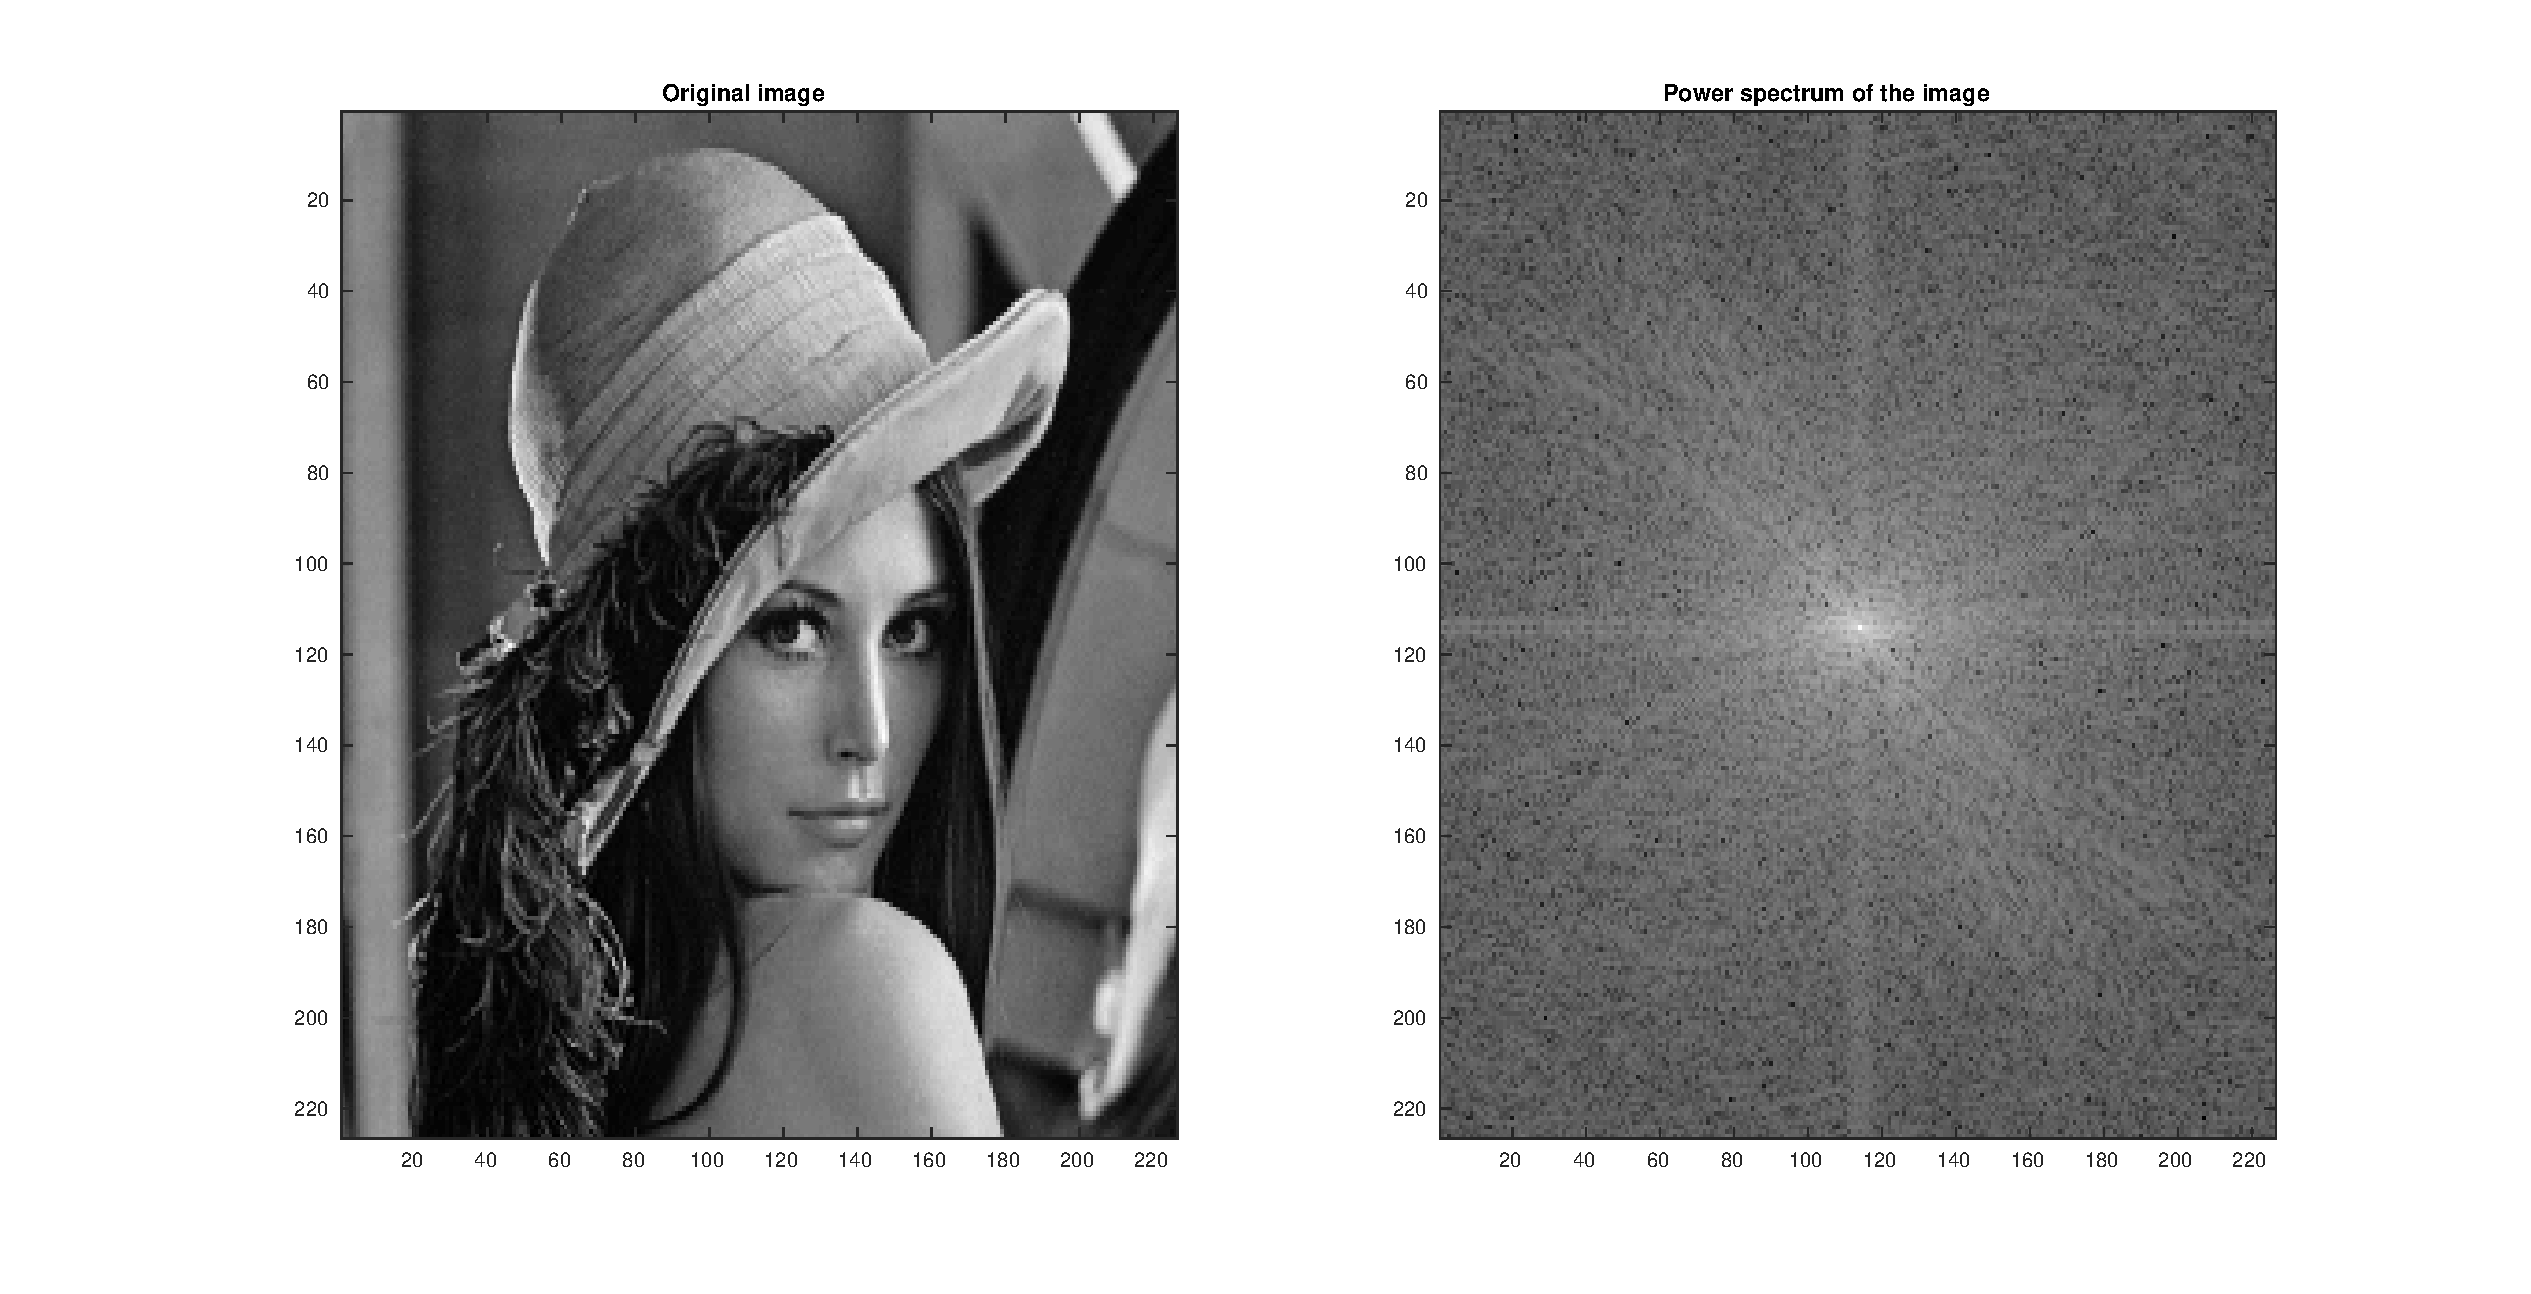
\includegraphics[scale=0.5]{fig1}
  \caption{Bipartite graph with vertex set $S\cup J$ with edge set $\{xj :x\in S, j\in J,
  x\in A_j\}$.}
  \label{fig1}
\end{figure}
where $\mathcal{A}=(A_1,A_2,A_3)$ with $A_1=\{1,2,3\}$, $A_2=\{2,3,4\}$ and
$A_3=\{4,5,6\}$.

\subsection*{(b)}
The geometric representation for $M[\mathcal{A}]$ is given by finding the transversal
matroid in Figure \ref{fig1}. The set $\{5,6\}$ is a circuit of size $2$ and $\{1,2,3\}$
is a circuit of size $3$. There is not circuit including $4$, so we put that by itself.
This gives us the following representation:
\begin{figure}[H]
  \centering
  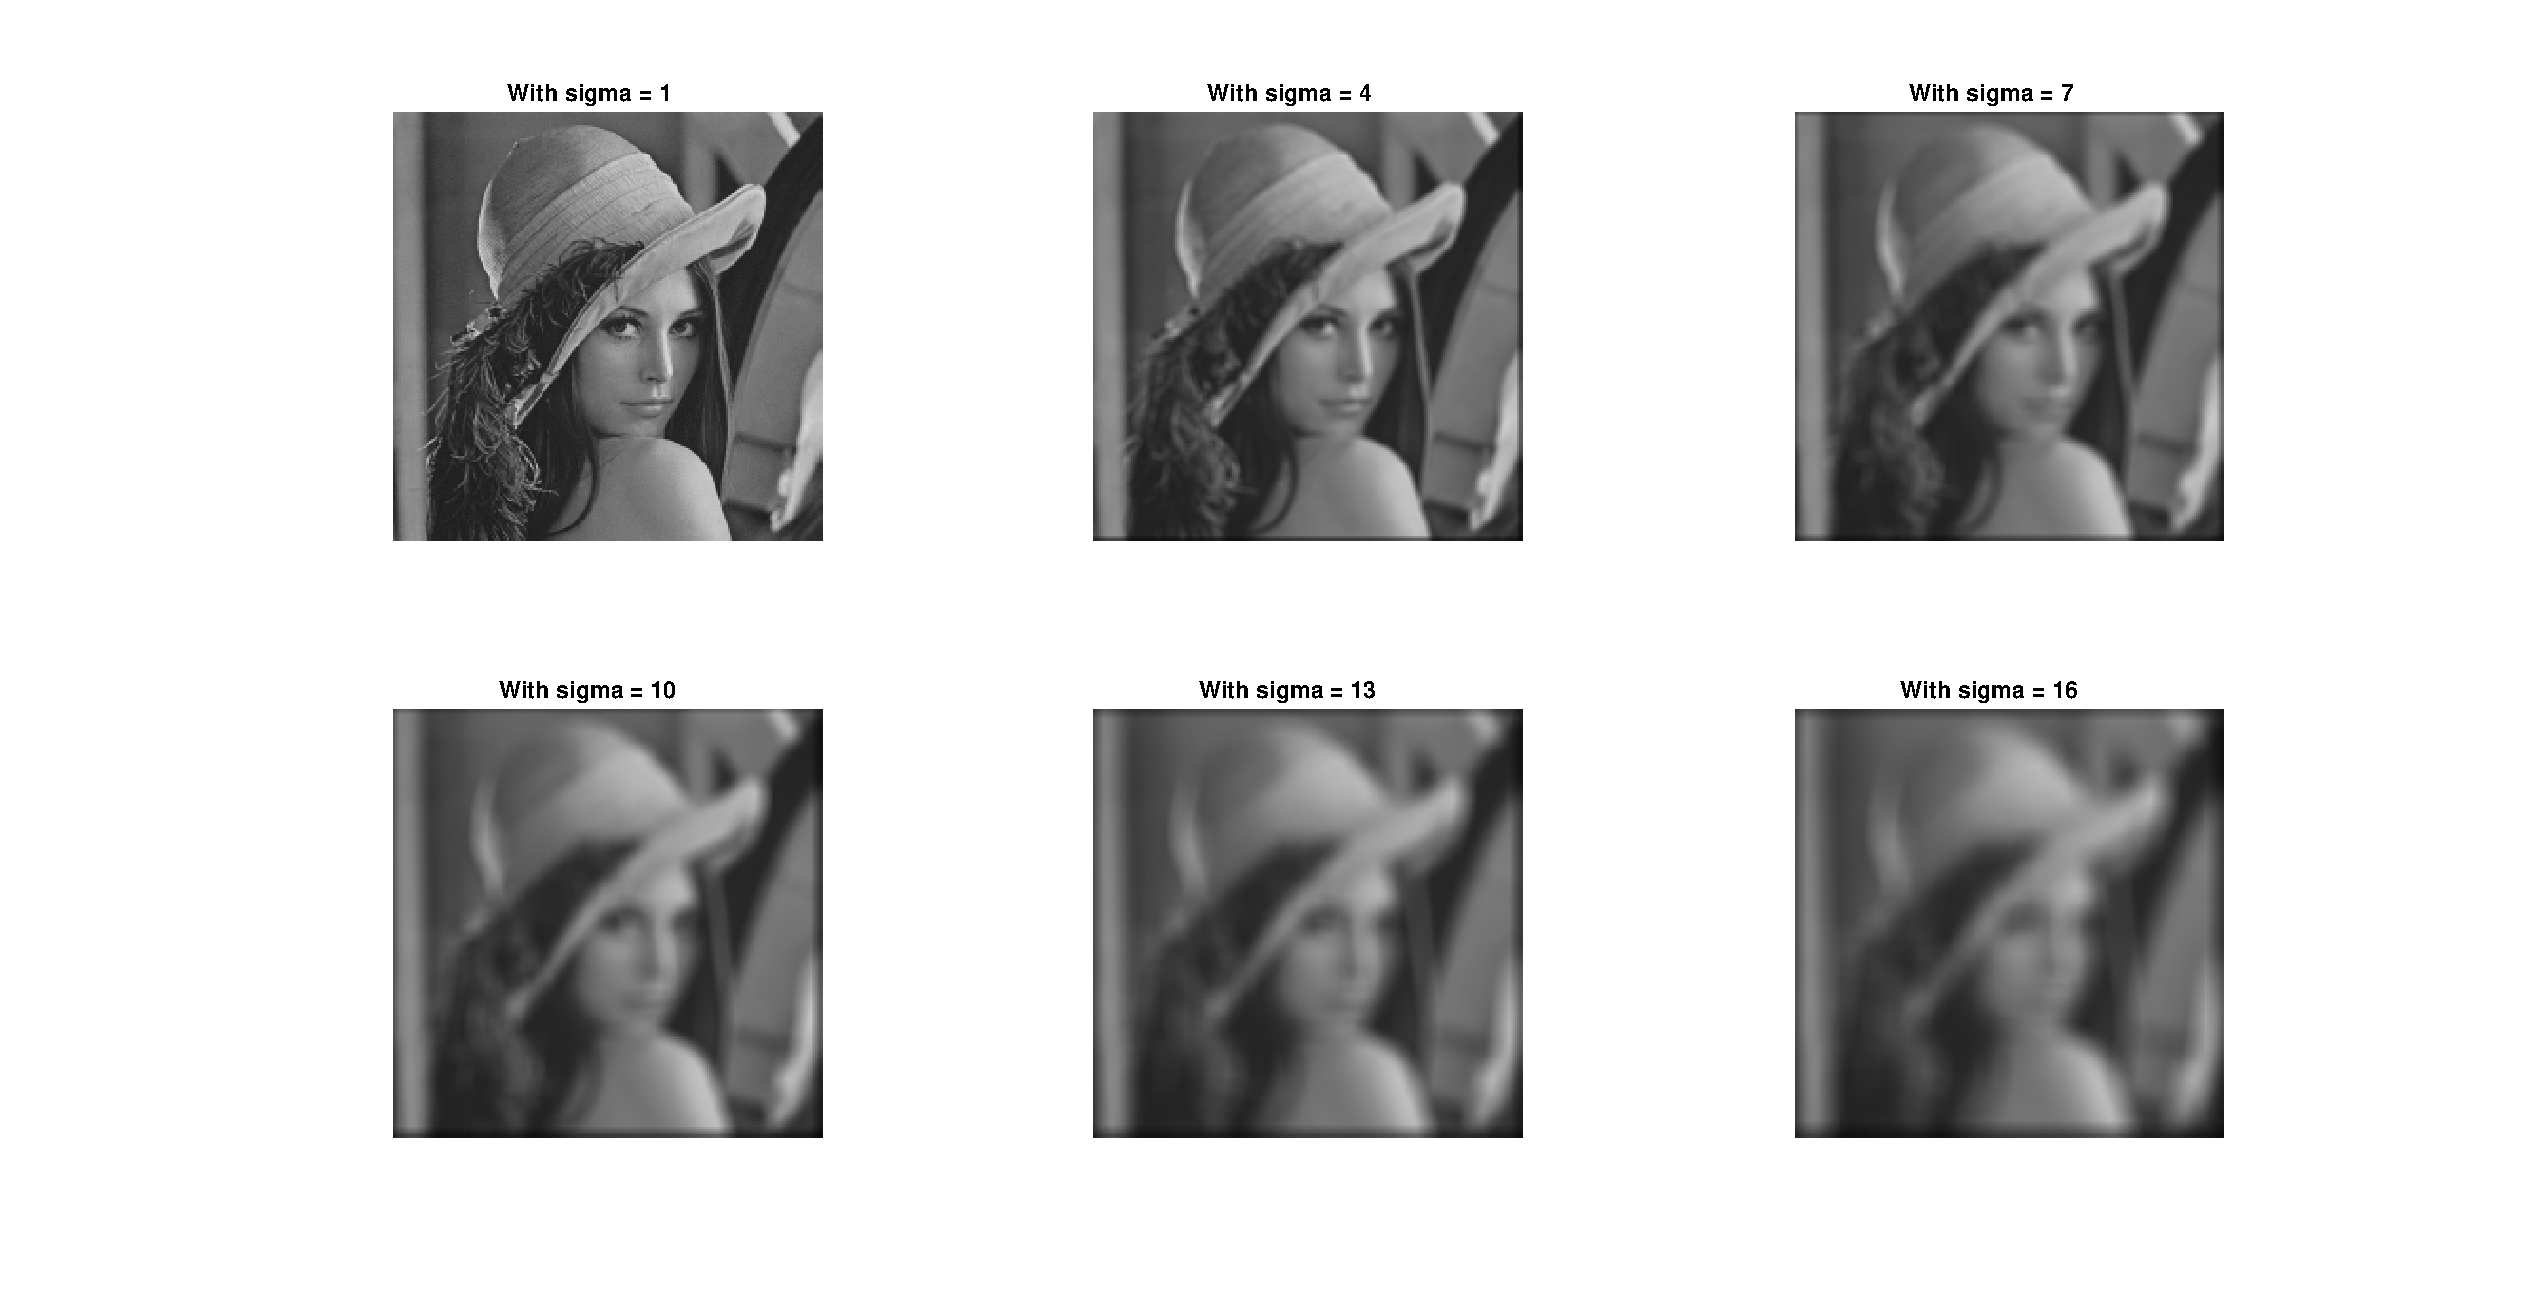
\includegraphics[scale=1]{fig4}
  \caption{Geometric representation of the transversal matroid from Figure \ref{fig1}.}
  \label{fig4}
\end{figure}
Which can easily be verified.

\section*{Question 4}
We give the subset which are independent:
\begin{align*}
  \mathcal{A}=&\{\{1\},\{2\},\{3\},\{4\},\{5\}, \\
              &\{1,2\},\{1,3\},\{1,4\},\{1,5\},\{2,3\},\{2,4\},\{2,5\},\{3,4\},\{3,5\},\{4,5\},
  \\
&\{1,2,4\},\{1,2,5\},\{1,3,4\},\{1,3,5\},\{2,3,4\},\{2,3,5\},\{2,4,5\}\}
\end{align*}
There are no independent set of size $4$ as it is drawn in one plane.

\section*{Question 6}
\subsection*{(a)}
Let $M$ be the matroid on $E=\{1,2,3\}$ with $\mathcal{I}=\{\emptyset, \{1\},\{2\}\}$,
then if we have the two subset $X=\{1,3\}$ and $Y=\{2,3\}$, (\textbf{R3}) gives us:
\begin{align*}
  r(X\cup Y)+r(X\cap Y)&=1 \\
                       &< r(X)+r(Y) \\
                       &= 2
\end{align*}
So equality does not always hold in (\textbf{R3}) for this particular matroid.

\section*{Question 7}
If $M$ is a uniform matroid $U^m_n$, we know by definition a subset is a basis if it has
$m$ elements and a circuit if has $m+1$ elements. Since the rank of any matroid is the
size of a basis, that means we cannot have a circuit of size less than or equal to $r(M)=m$ as it would be a basis. \\
If a matroid has no circuits of size less than $r(M)+1$, then any subset of size $r(M)$
must be independent. Again, since rank is equal to the size of a basis, any subset of
size $r(M)$ is also a basis. This means any subset of size $r(M)+1$ must be a circuit,
which is exactly the definition of a uniform matroid.

\end{document}
